\section{Move Order \& Picking Phase}
\subsection{Explanation of Move Order - ABBA} \label{ABBA}

\begin{wrapfigure}{r}{0.35\textwidth}
    \centering
    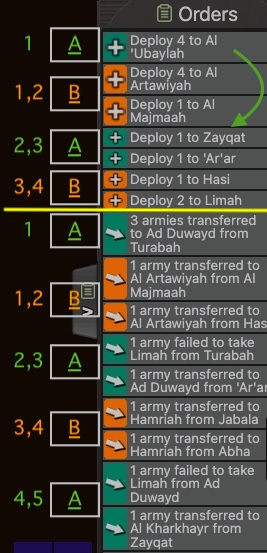
\includegraphics[width=0.25\textwidth]{Images/moveorder.jpg}
    \caption{ABBA applied}
    \label{ABBA_image}
\end{wrapfigure}

In accordance with \href{https://www.warzone.com/wiki/Move_Order}{Warzone Wiki Move Order Explanation}, in a Warzone 1vs1 game between player A and player B, and under the assumption that player A has the first move, the move order alternates as $\text{ABBAABBAA}\dots$. This sequence can be described as follows:

\begin{itemize}
    \item Player A executes their $1^{\text{st}}$ move.
    \item Player B executes their $1^{\text{st}}$ and $2^{\text{nd}}$ moves consecutively.
    \item Player A executes their $2^{\text{nd}}$ and $3^{\text{rd}}$ moves consecutively.
    \item Player B executes their $3^{\text{rd}}$ and $4^{\text{th}}$ moves consecutively.
    \item Player A executes their $4^{\text{th}}$ and $5^{\text{th}}$ moves consecutively.
    \item Player B executes their $5^{\text{th}}$ and $6^{\text{th}}$ moves consecutively.
    \item And so on, following the $\text{ABBA}$ pattern, with an example at Figure \ref{ABBA_image}.
\end{itemize}

This pattern ensures that player A and player B alternate moves, with each player receiving consecutive moves in pairs after the first move by player A. The sequence $\text{ABBA}$ then continues cyclically.
\\
\\
Of course, in the opposite case that player B has first move, then the move order follows the inverse pattern $\text{BAABBAABB} \dots$. The ABBA algorithm determines not only the order of moves but also the order of deployments, without exception. The arising question regarding the above rule, how is it decided which player moves first each turn. The answer to that question relies on the 3 different settings of implementation one can find upon creating a game. Needless to say, each game follows exactly 1 of the settings below:
\begin{enumerate}
    \item Random Move Order \ref{random_move_order}
    \item Cyclic Move Order \ref{cyclic_move_order}
    \item No-Luck Cycle Move Order \ref{noluck_cycle}
\end{enumerate}

%%%%%%%%%%%%%%%%%%%%%%%%%%%%%%%%%%%%%%%%%%%%%%%%%%%%%%%%%%%%%%%
%%%%%%%%%%%%%%%%%%%%%%%%%%%%%%%%%%%%%%%%%%%%%%%%%%%%%%%%%%%%%%%

%%%%%%%%%%%%%%%%%%%%%%%%%%%%%%%%%%%%%%%%%%%%%%%%%%%%%%%%%%%%%%%
%%%%%%%%%%%%%%%%%%%%%%%%%%%%%%%%%%%%%%%%%%%%%%%%%%%%%%%%%%%%%%%

